\section{Introduction}

The most efficient cryptographic protocols are symmetric, in that they use a single shared key.
To securely exchange a shared key, public key cryptography is used. Public key cryptography
relies on a public key for encryption and a private key for decryption, as first described by
Diffie and Hellmann.

\begin{figure}[htb]
	\centering
	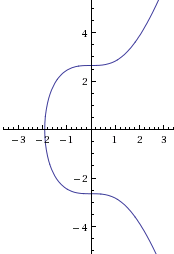
\includegraphics[width=0.30\textwidth]{introduction/secp256k1-graph}
	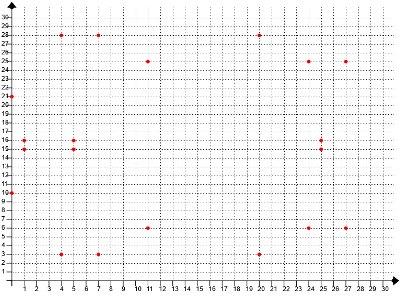
\includegraphics[width=0.59\textwidth]{introduction/secp256k1-graph-over-field-p31}
	\caption{hello http://www.graui.de http://www.wolframalpha.com}
	\label{fig:graphs}
\end{figure}

Note: Extensive introduction of elliptic curves. Introduce abbreviation "ECC". Three images:
(1) elliptic curve; (2) elliptic curve in finite field; (3) integers of elliptic curve in finite
field.

Note: Add something about patent problems (not many free implementations exist!)

Note: Add paragraph on different types of curves (Weierstrass, Montgomery).

Elliptic curves provide a new mathematical model that can be used as the basis for cryptography,
as they allow for the creation of one-way "trapdoor" functions to be constructed (Section
\ref{sec:math_encryption}).

In 1995, ElGamal described a simple (as in simply brilliant) public key cryptosystem that can be adapted
to use elliptic curves (Section \ref{sec:math_encryption_elgamal}). This system relies on the ability to
encode messages as points on an elliptic curve (Section \ref{sec:math_encoding}). Other cryptosystems,
such as ECIES, are \emph{hybrids}, using the asymmetric properties of elliptic curve-based cryptography,
as well as a symmetric cryptosystem. An implementation of ECIES using AES as the underlying symmetric
system is shown (Section \ref{sec:math_encryption_ecies}).

This paper describes the structure of \emph{OpenECC}, an open-source implementation of the functionality
described in the mathematical foundation section. \emph{OpenECC} has been developed concurrently with the
production of the paper, and is used as a basis for performance measurements, comparing the different constructs
with each other, measuring which are the most efficient (Section \ref{sec:performance}).

The implementation is modular, allowing for different curves and encryption schemes to be swapped in and out
rapidly (Section \ref{sec:implementation_structure}). It also provides a readable syntax that makes it more easily
understandable than available alternatives, such as Bouncy Castle (Section \ref{sec:implementation_usability}).

While \emph{OpenECC} implements the constructs used specifically in elliptic curve cryptography it relies on certain
external constructs. The elliptic curves rely on Bouncy Castle's implementation of finite fields, which makes comparisons
limited to the elliptic curve layer more accurate (such comparisons are performed in Section \ref{sec:performance_bouncycastle}).
The ECIES implementation relies on the native Rijndael implementation that ships with C\#.

Note: Add source to paragraph below! Or consider removing the paragraph...

Comparisons of the security provided per key-length for different cryptographic algorithms exist\footnote{Source?!}. With
most mathematical operations - including those used in ECC - several performance optimizations exist over the naïve
implementation. The performance of traditional public-key cryptography implementations has been continuously improved
since its inception. To understand whether ECC is feasible as an alternative to traditional cryptography, the performance
of ECC must be evaluated in relation to that of traditional public-key cryptography implementations.

Note: There should be hints at the findings of the report here! (Performance...)